\let\textcircled=\pgftextcircled
\chapter{TWO}
\label{chap:intro}
\section{Machine Learning}
Arthur Samuel defines Machine learning as follows : " A field of study that gives computers the ability to learn without being explicitly programmed."\cite{art4} \\

Machine learning is a scientific field, and more specifically a subcategory of artificial intelligence. It consists of letting algorithms discover “patterns”, namely recurring patterns give computers the ability to learn from data sets, i.e. improve their performance to be able to solve tasks without being programmed already.
a data can be numbers, words, images, statistics, Machine learning also helps us find solutions to many problems in vision, speech recognition, and robotics\cite{book2}
\subsection{Machine learning concepts }
Some concepts of machine learning needs to be explained first:
\subsubsection{Splitting data}
While constructing the model, the data needs to be splited to avoid overfitting into two three parts, training test,validation and test set 
\begin{itemize}
    \item raining set The portion of data used for training the model, and need to take big part of the split. In this part of the split, the class labels are known for the data objects.  
    \item Validation set The validation set is a set of data, separate from the training set, that is used to validate our model during training. This validation process helps give information that may assist us with adjusting our hyperparameters.
    \item Test set The test set is a set of data that is used to test the model after the model has already been trained. The test set is separate from both the training set and validation set. The test set should not be labeled. 

\end{itemize}
\subsubsection{Underfitting and overfitting}
A model that would just repeat the labels of the samples that it has just seen would have a perfect score but would fail to predict anything useful on yet-unseen data, this called overfitting. If the model fits perfectly the training data, the predictive accuracy on new data must not necessarily be good. One major problem of machine learning is overfitting , is one the modal perfectly knows how to class the data points during the training, but the mis-classified data during the test is very high. which means that the model is suitable only for the data he was trained on. 
\subsubsection{Underfitting}
in the other side when the model isn’t complex enough to be able to map and represent the data while training, and can’t generalize the new data one solution is proposed to solve this problem is regularization.\cite{book3}
\begin{figure}[!h]
    \centering
    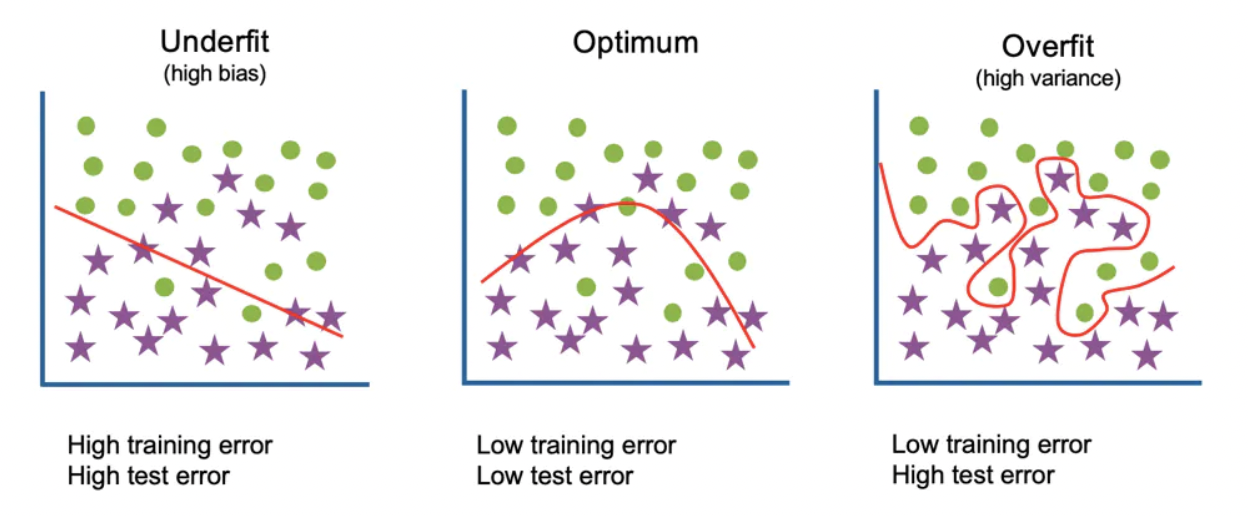
\includegraphics[width=1\textwidth]{chapters/chapter02/fig02/overfiting.png}
    \caption{Underfitting and overfitting in classification , the third plot in the left is using all the parameters of the model, and this will lead to adapt the exact parameters of the the exact data point and won’t be able to generalize new data
}
    \label{fig:my_label}
\end{figure}
\subsubsection{Regularization}
Regularization is the process of generalizing the model and make it more representive to the data, used to prevent overfitting and co-adaptations of model’s connection. each algorithm of machine learning should have a regularization parameters, many ways to do regularization will be described the next chapter.[ Andrew NG Machine learning course in corsera,https://www.coursera.org/learn/machinelearning.
Last accessed on 10-06-2019.]
\subsubsection{Model validation}
one more way to prevent overfitting , validation is the task of demonstrating that the model is a reasonable representation of the actual system: that it reproduces system behavior with enough fidelity to satisfy analysis  \cite{art5}
there are many ways to validate the model, here’s one of them:
\rule[0.5ex]{\linewidth}{1pt}\\
\textbf{Algorithm 1: }K-fold cross validation algorithm \\
\rule[0.5ex]{\linewidth}{1pt}
\begin{enumerate}
    \item Split the dataset into training set and test set
    \item The training set is split into k smaller sets
    \item A model is trained using K-1 of the folds as training data
    \item The remain part of data is used for validation
    \item This operation is repeated K times.
    \item The performence is measured by the average of values returned in the loop
\end{enumerate}
\rule[0.5ex]{\linewidth}{1pt}
\begin{figure}[!h]
    \centering
    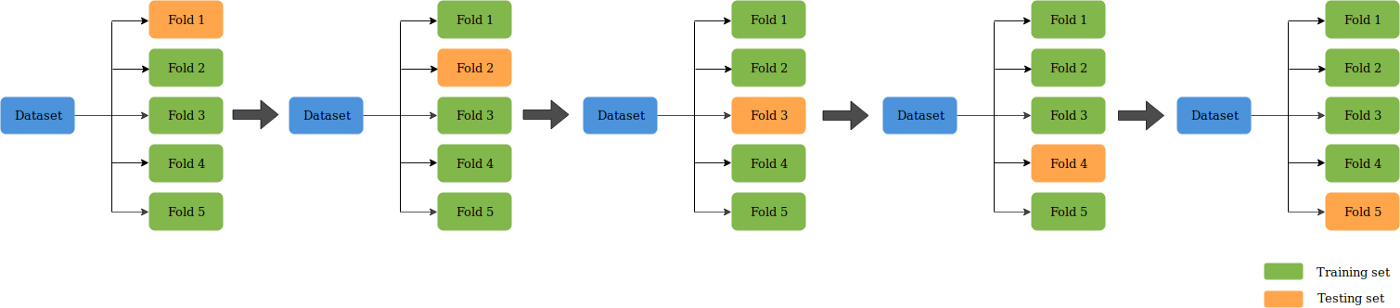
\includegraphics[width=17cm,height=5.5cm]{chapters/chapter02/fig02/kfold.png}
    \caption{Caption}
    \label{fig:my_label}
\end{figure}
\subsection{Supervised learning}
Supervised learning is the machine learning task of learning a function that maps an input to
an output based on example (xi,yi), where xi is the input and yi the corresponding target class \cite{art5}
\subsubsection{SVM}
Stands for Support Vector Machines was first proposed by V.Vapnik \cite{vapnik},is one of
the most powerful and popular machine learning methods that can be used in either
classifications and regression tasks, it’s commonly used in classification problems. SVM
can perform in both linear separable and non separable data , in the second case, SVM
uses Kernels to transfer the data-points into a higher dimensional space where they can
be linearly separable.
\begin{figure}[!h]
    \centering
    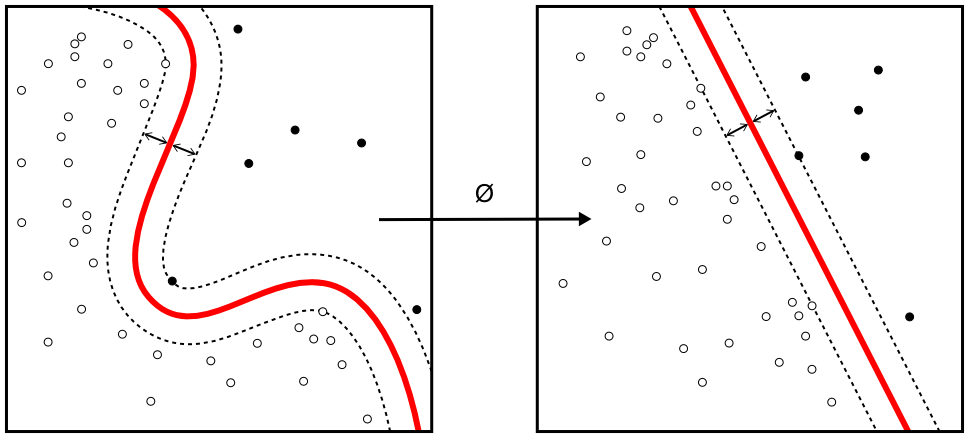
\includegraphics[width=1\textwidth]{chapters/chapter02/fig02/svm.png}
    \caption{SVM in linearly seperable data on the right, the discantious lines are the
margins, the data ponints on these lines are called the support vectors, the goal is to
maximize these margins, on the left side, the kernel trick of SVM when the data in
non-linear seperable.
}
    \label{fig:my_label}
\end{figure}
SVM simultaneously minimize the empirical classification error and maximize the
geometric margin. So SVM called Maximum Margin Classifiers \cite{book5} SVM parameters
such as kernel parameters and penalty parameter have a great influence on the complexity
and performance of predicting models.
\paragraph{Related works using SVM }
\begin{itemize}
    \item Padol, P. B \textit{et al} \cite{art6}  proposed a system  to aid in the detection and classification leaf diseases of grape using SVM classification technique. First the diseased region is found using segmentation by K-means clustering, then both color and texture features are extracted. Finally classification technique(svm) is used to detect the type of leaf disease.\\
    
    The proposed work focused on recognition and classification of fungal disease like Downy Mildew and Powdery Mildew ,  total 137 grape leaf images (containing both initial stage as well as final stage images) are used out of which 75 images are Downy leaf images and 62 are Powderly leaf images. For training phase 60 Downy and 50 Powderly images are used and 15 Downy and 12 Powderly are used for testing.\\ \vspace{4mm}
    The proposed system can successfully detect and classify the examined disease with accuracy of 88.89%.\\
    
    \item S. Arivazhagan \textit{et al} \cite{art7} proposed  an application of texture analysis in detecting and classifying the plant leaf diseases.\\
    About 500 plant leaves of 30 different native plant species of Tamil Nadu(india) have been collected for this work. the proposed algorithm was tested on ten species of plants namely banana, beans, jackfruit, lemon, mango, potato, tomato, and sapota\\ \vspace{4mm}
    The classification gain obtained by Minimum Distance Criterion is 86.77\%. The detection accuracy is improved to 94.74\% by SVM classifier
\end{itemize}
\subsubsection{Random Forest}
Random Forest or random decision forests, it is a supervised classification algorithm consisting
of many decisions trees, meaning the approach generate a random forest which is a combination
of decision trees models.
\begin{figure}[!h]
    \centering
    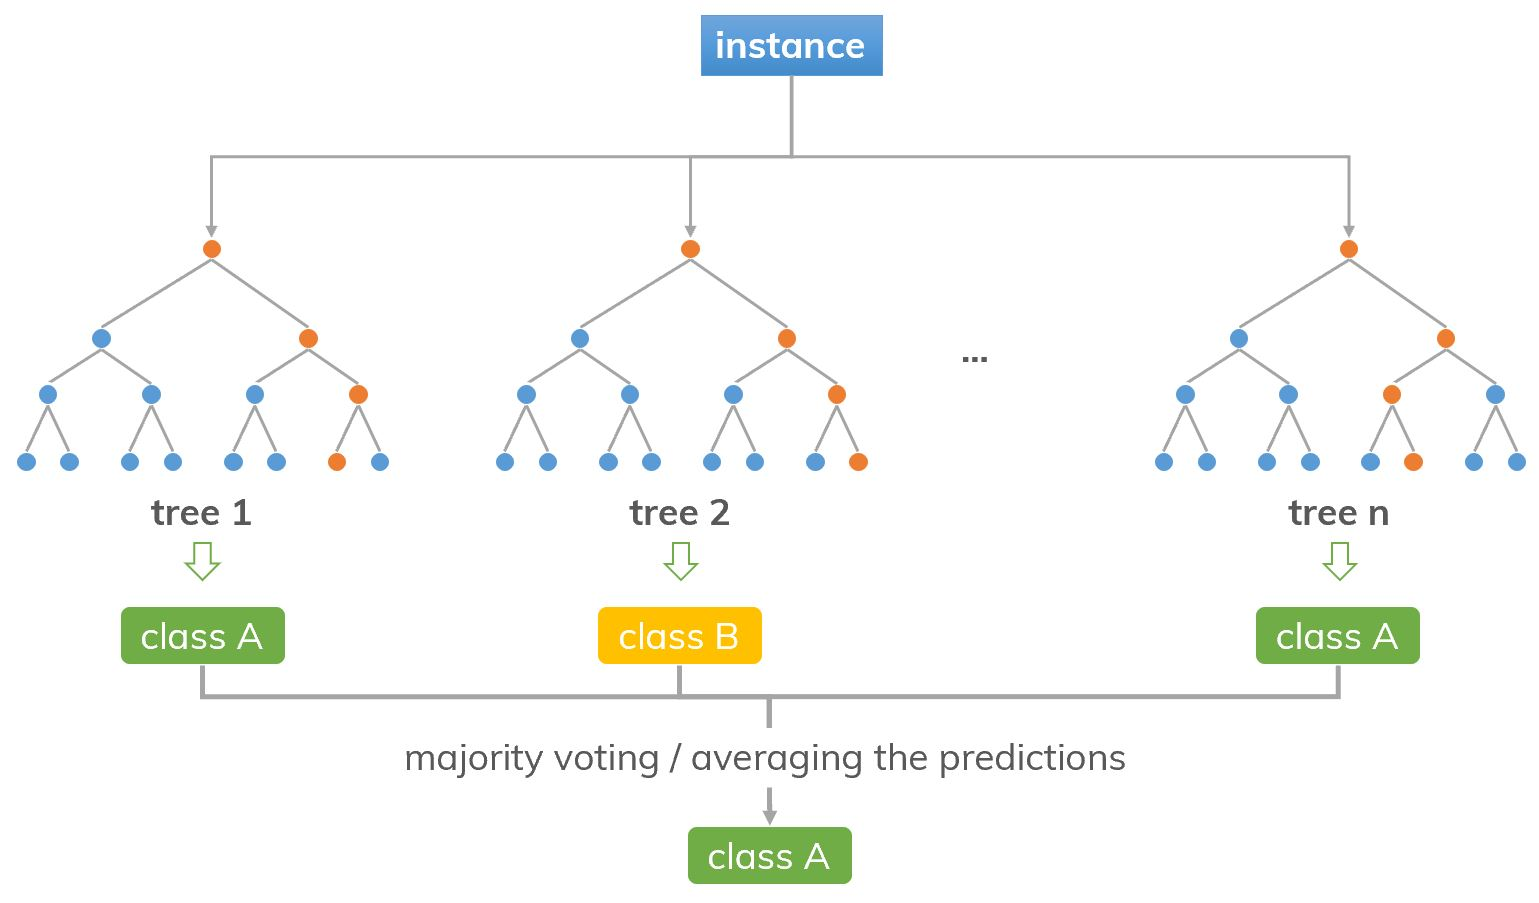
\includegraphics[width=0.8\textwidth]{chapters/chapter02/fig02/rf1.jpg}
    \caption{Random forest classifier}
    \label{fig:my_label}
\end{figure}

\paragraph{Related work using random forest}
\begin{itemize}
    \item S Ramesh \textit{et al} \cite{art8}  propose a methodology based on the algorithm Random Forest in identifying between healthy and diseased leaf ,this algorithm are flexible in nature and can be used for both classification and regression techniques.\\\vspace{4mm}
    The algorithm was contrasted with other machine learning models for accuracy. Using Random forest classifier, the model was trained using 160 images of papaya leaves. The model could classify with approximate 70 percent accuracy. The accuracy can be increased when trained with vast number of images
Compared to other machine learning techniques like SVM (Accuracy 40.33 \%), Naïve bayes (Accuracy 57.61 \%),  logistic regression(Accuracy 65.33 \%),  Random forests gave more accuracy (70.14 \%), with less number of image data set.

\item CHAUHAN, Ms Deepika, \textit{et al.} \cite{art9}.The  proposed  method  was  applied  using  image  data  with  a  label  to  train  the  separation model with various techniques such as  KNN(Accuracy 72.16\%),NB(Accuracy 74.35\%) , DT(Accuracy 73.35\%), SVM(Accuracy 76.16\%), and RF in the maize disease  detection database and finds that  the RF(Accuracy 80.68\%) classification process is better than other classification  methods.\\ \vspace{4mm}
maize  data  sets  are  divided  into  training  data  (90\%)  and  test  data  (10\%).  The maize plant disease  database contains a  total of 3,823 photographs andfour category labels.  The  details of the section  label  information  about  maize  disease  data  are  as  follows:  gray  area,  common  rust,  damage  to  thenorthern leaves,  and healthy 513, 1192, 985, and 1162, respectively.
\end{itemize}
\subsubsection{Logistic regression}
Is supervised classification algorithm used to classify data to a discrete set of classes(
classes are already determined ), by using sigmoid function to return a probability
value ( between 0 and 1 ) which can be used to map the instance into its corresponding
class. If there are many classes to assign, Logistic regression applies One Vs All approach.\\

\textbf{One Vs All classification : }It is a technique applied by Logistic regression to classify the
data ,in the case of many classes should be assign.
One-Vs-All is a strategy that involves training a single classifier per class, with the samples of
that class as positive samples and all other samples as negatives.
\newpage
\begin{figure}[!h]
    \centering
    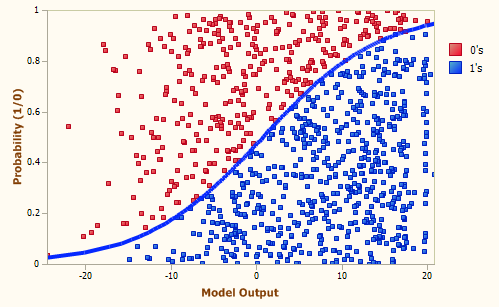
\includegraphics[width=1\textwidth]{chapters/chapter02/fig02/lr.png}
    \caption{Logistic regression example}
    \label{fig:my_label}
\end{figure} 
\begin{figure}[!h]
    \centering
    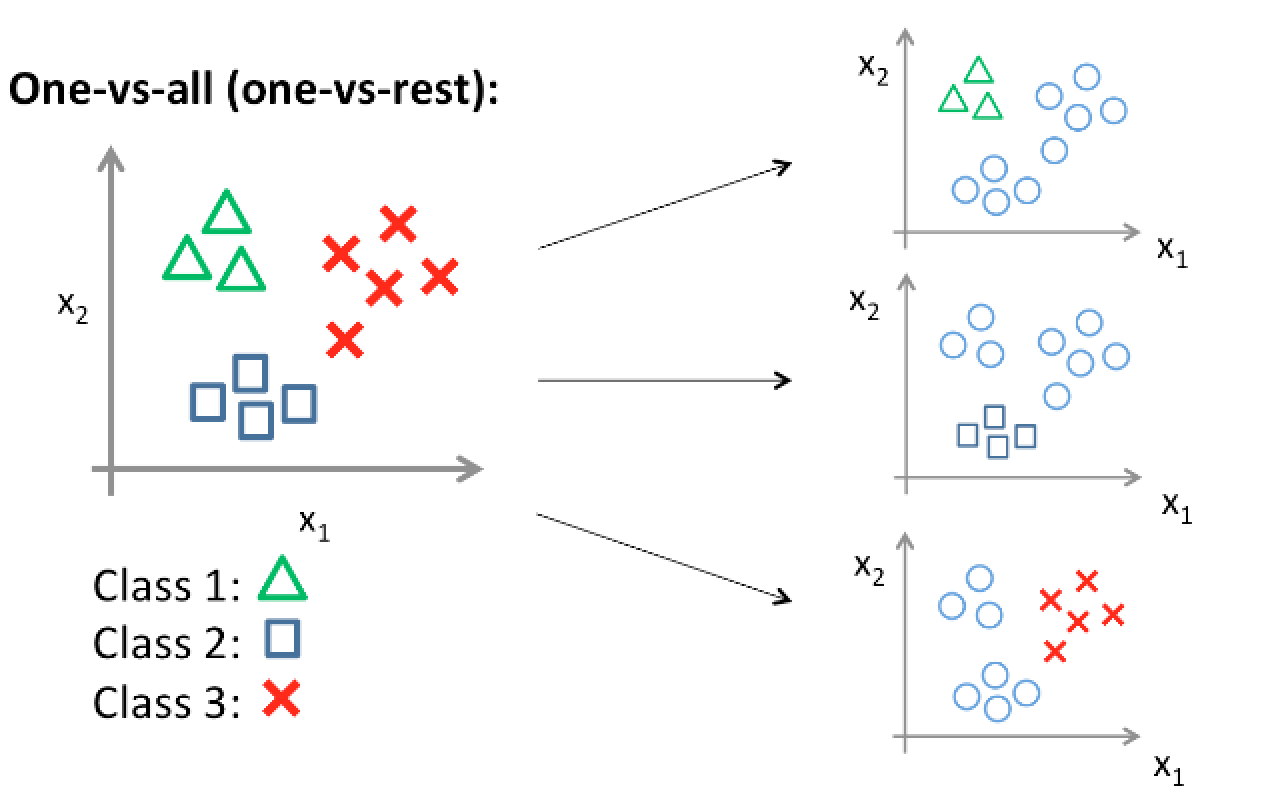
\includegraphics[width=0.9\textwidth]{chapters/chapter02/fig02/ova.png}
    \caption{One Vs All classification}
    \label{fig:my_label}
\end{figure} 
\newpage
\paragraph{Related works using Logistic regression :}
\begin{itemize}
    \item According to  Mila, A. L \textit{et al} \cite{art10} Logistic regression is used widely in epidemiological research, where the binary response usually is the presence or absence of a disease, In this case it was used to estimate the probability of soybean stem rot  prevalence with historical disease data from four states of the north-central region of the United States.\vspace{4mm} \\
    Two models were developed: model I used spring (April) weather conditions and model II used summer (July and August) weather conditions as input variables. Both models had high explanatory power (78.5 and 77.8\% for models I and II, respectively).

    \item D Tiwari \textit{et. al} \cite{art11} have used the logistic regression as classifier for a proposed model , 2152 images of potato leaves were taken from a plant village dataset which comprises 1000 images of early blight,1000 images of late blight, and 152 of healthy images of potato leaves. Dataset is divided into two parts: the training part comprises 1700 images(70\%) and the test part contains 452 images(30\%). Various pre-trained models like inceptionV3 , VGG16 , and VGG19  are used for feature extraction among which VGG19 gave the optimal result.\vspace{4mm}
    Multiple classifiers namely KNN , SVM , Neural Network , and logistic regression are used for classification. Among which Logistic Regression gives the state-of-the-art solution with a classification accuracy of 97.7\%

\end{itemize}
\subsubsection{KNN}
kNN Stands for k Nearest Neighbors, is a popular classification approach. The simple, the new data point is classified according to the classes of the k nearest neighbors to it. The K nearest refers to the similar or close (in term of distance ) points to that data, there are many methods to calculate this distance, Euclidian distance , Jaccard distance, Manhattan .. and K refers to the number of neighbors. After calculating the distance from this point to its neighbors, the label of this data point is maintained corresponding to the labels of the k nearest neighbors.\cite{book5}
\begin{figure}[!h]
    \centering
    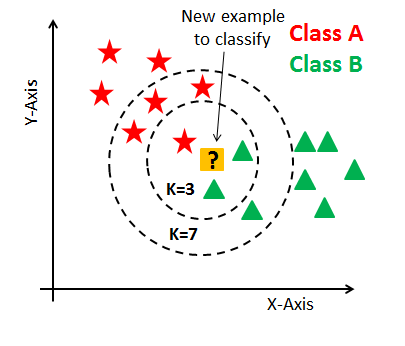
\includegraphics[height=4cm,width=0.37\textwidth]{chapters/chapter02/fig02/knn.png}
    \caption{Knn example with k=3, k=7}
    \label{fig:my_label}
\end{figure}
\paragraph{Related work using KNN}
\begin{itemize}
    \item Ramcharan, Amanda,\textit{ et al} \cite{art12} proposed a method  to aid in the detection and classification leaf diseases using KNN classification technique. The method is divided into two phases: the training phase and the testing phase. The training and testing phases comprise of five fundamental stages which are image acquisition, color conversion, color segmentation, morphological operation, and feature extraction. K-nearest neighbor classifier is taken out for color image segmentation.\vspace{4mm} \\
    The proposed work focused on recognition and classification of five disease like Alternaria alternata, anthracnose, bacterial blight, leaf spot, and citrus canker leaf, total 237 leaf images are used out of which Among these images, total 177 leaf images are Alternaria alternata, anthracnose, and bacterial blight disease affected and each type has 59 leaf images. Other, 60 images are leaf spot and canker affected where each disease type image numbers are 30.\vspace{4mm} \\
    The proposed method can successfully detect and classify the examined disease with accuracy of 96.76 \%.
    \item Vaishnnave, M. P., \textit{et al} \cite{art13} proposed a method  to aid in the detection and classification leaf diseases using KNN classification technique. The developmental method of the proposed scheme includes two components Disease Identification: Identification of disease affected. Disease Management: Remedial measure for disease. \vspace{4mm}\\
    In the selected 250 images, 45 denoised images are trained with KNN classifier and their features are in use for pattern matching; remaining 105 images are used for testing. They categorized only 4 dissimilar disease with of efficiency.

\end{itemize}
\subsubsection{Decision Tree}
 Is a supervised algorithm used for classifications, in some cases can be used for regression, it classifies the input data by sorting them based on attribute or feature values. The decision tree model is composed of nodes, each node represents a feature in an instance that we aim to classify, and each branch represent the value of the node. Instances are classified starting at the root node and sorted based on their feature values. \cite{art5} \newpage
 \begin{figure}[!h]
     \centering
     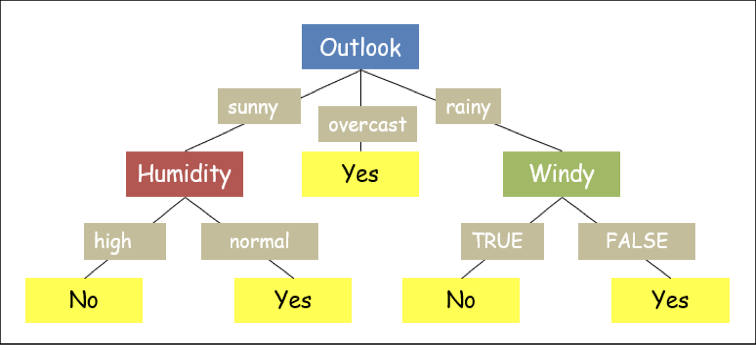
\includegraphics[width=1\textwidth]{chapters/chapter02/fig02/dt.png}
     \caption{An example of a decision tree, this diagram is used by Tom Mitchel In his paper \cite{art14} he describes his ID3 algorithm, nodes represent attribute values Branches are tests, the last node explain if the person plays tinis or not}
     \label{fig:my_label}
 \end{figure} 
 
\paragraph{Related works using decision tree}
\begin{itemize}
    \item Rajesh, B., M. Vishnu Sai Vardhan, and L. Sujihelen. \cite{art15} proposed a system to aid in the detection and classification leaf diseases using Decision Tree classification technique. The main purpose of this proposed system is to detect the leaf disease and identify what type of disease. The proposed work uses a decision tree to identify the leaf disease. The proposed work is based on the morphological characteristics of plant leaves. \vspace{4mm}\\
    The dataset contains more than 1000 images of the leaf are 145 Healthy images, 200 Late Blight images, 100 Bacterial Spot images, 355 Yellow Curl Virus images and 200 Anthracnose images.\vspace{4mm} \\
    The proposed system can successfully detect and classify the examined disease with accuracy of 96 \% for Tomato and 95 \% for Lemon.
    \item Ahmed, Kawcher, \textit{et al} \cite{art16} proposed a system to aid in the detection and classification leaf diseases using Decision Tree classification technique. The main idea of this work is to create a rice leaf disease detection model using machine learning algorithms that can be helpful for disease recognition. \vspace{4mm}\\
    The dataset has 480 images for three types of rice leaf disease, was divided into two parts: training and test sets where training data contains 432 instances (90\% of the 480) and test data contains 48 instances (10\% of the 480).\vspace{4mm}\\
    The proposed system can successfully detect and classify the examined disease with accuracy of 94.9074 \% for training set and 97.9167 \% for testing set.


\end{itemize}
\subsubsection{Naïve Bayes}
Bayesian classifiers are statistical classifiers. They can predict class membership probabilities, such as the probability that a given sample belongs to a particular class. Bayesian classifier is based on Bayes’ theorem. Naive Bayesian classifiers assume that the effect of an attribute value on a given class is independent of the values of the other attributes. This assumption is called class conditional independence. It is made to simplify the computation involved and, in this sense, is considered ”naive”. \cite{art17}
\begin{figure}[!h]
    \centering
    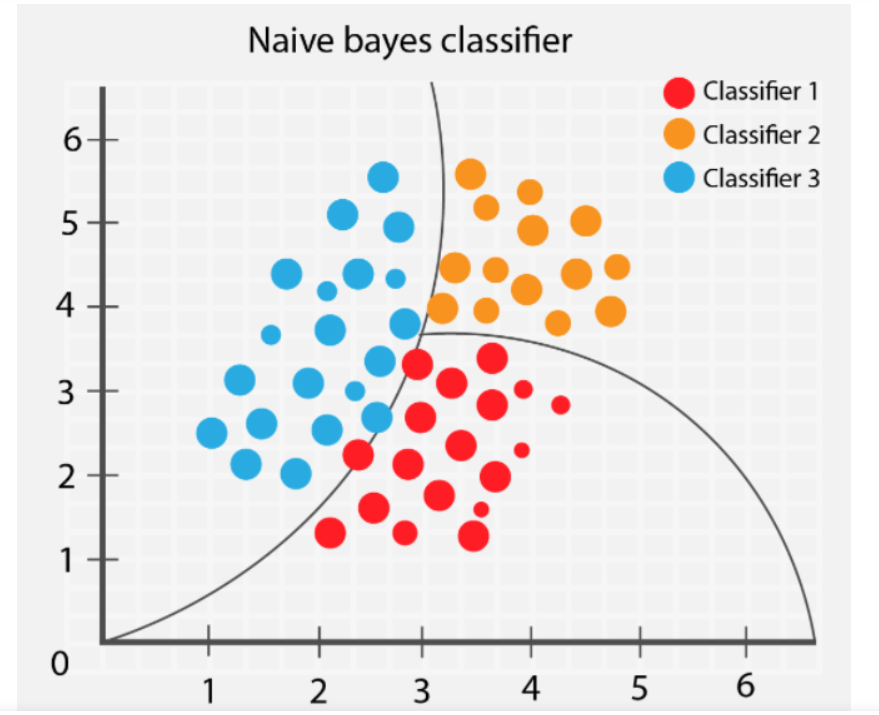
\includegraphics[width=0.8\textwidth]{chapters/chapter02/fig02/nb.png}
    \caption{Naïve Bayes Classifier}
    \label{fig:my_label}
\end{figure}
\paragraph{Related Works using Naïve Bayes}
\begin{itemize}
   \item Panigrahi, Kshyanaprava Panda,\textit{et al} \cite{art19} proposed a method to aid in the detection and classification leaf diseases using Naïve Bayes classification technique.
    The proposed method has several components such as image acquisition, image preprocessing, image segmentation, feature extraction, classification, and performance evaluation. \vspace{4mm}\\
    The proposed method can successfully detect and classify the examined disease with accuracy of 77.46 \%.

\end{itemize}


\subsection{Unsupervised learning}
One important type of machine learning when the data is unlabeled and there is
no priori identified classes, then it aims to find in the collection of data if there are
clusters, groups to be discovered. usually members of same cluster or group are similar
to each other and dissimilar to member of other groups. The process is simple , we try
to maximize the distance between the clusters and minimize the distance between the
members of each cluster.
There are different objectives in unsupervised learning problems, such as clustering and
visualization. example: Kmeans, Fuzzy c means , HCA. For visualization, the data is
projected down, from a high-dimensional space, to two or three dimensions like PCA.\cite{leg}
\subsubsection{}
\section{Deep Learning}
Deep learning, as a new area of machine learning research, is a process which allows the computer to learn to perform tasks which are natural for the brain like image recognition. Currently, deep learning (DL) methods have had a profound impact on computer vision and image analysis applications, such as image classification, segmentation, image completion and so on. Deep learning focuses on a specific category of machine learning called Artificial Neural Networks which is inspired by functionality of the human brain. Modern deep learning provides a very powerful framework for supervised learning. By adding more layers and more units within a layer, a deep network can represent functions of increasing complexity. Most tasks that consist of mapping an input vector to an output vector, and that are easy for a person to do rapidly, can be accomplished via deep learning, given sufficiently large models and sufficiently large datasets of labeled training examples. \cite{art20}
\subsection{Feedforward Networks}
Also named, Artificial Neural networks, have attracted considerable interest in recent
years due to their ability to learn complicated maps from examples, an ability termed
universal approximation. called networks because they are typically represented by
composing together many different functions
Called neural because they are loosely inspired by neuroscience. \cite{art20}
The learning algorithm must decide how to use those layers to produce the desired
output, but the training data does not say what each individual layer should do.
\subsection{Layers}
In this classic artificial neural networks there are many types of layers used in the
network, each type of layer is responsible for some computations.
\subsubsection{Input layer}
Input layer is the first layer in the neural network, composed of input neurons and
brings initial data to the hidden layers for further processing.
\begin{figure}[!h]
    \centering
    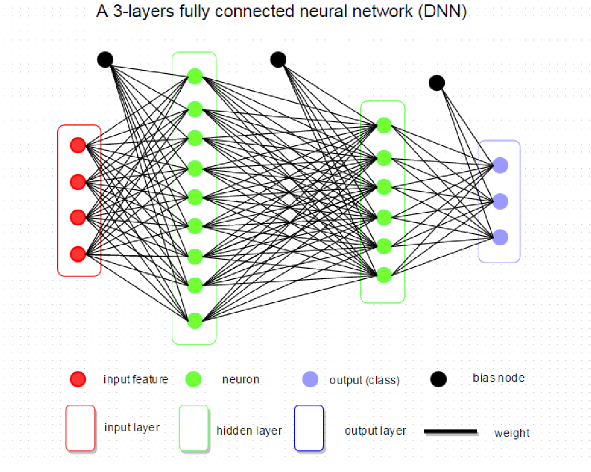
\includegraphics[width=0.9\textwidth]{chapters/chapter02/fig02/dnn.PNG}
    \caption{Artificial neural networks architecture}
    \label{fig:my_label}
\end{figure}
%image===========================================
\subsubsection{Hidden layer}
The layer or group of layers between the input and output layer. Deep learning is an
optimization problem looks for the optimal solution of a very complex problem, many of
these computations are made in the hidden layer(s).The choice of hidden layers depends
on the complexity of the data, when using a less complex data it’s recommended to use
few hidden layers, using many hidden layers in a simple problem can lead to overfitting,
and using simple architecture in complex problem leads to underfitting.
Each hidden layer of the network is typically vector-valued. The dimensionality of these
hidden layers determines the width of the model.
\cite{art20}
\subsubsection{Output layer}
Output layer is the last layer in neural network which produces the outputs of the
program, in classification tasks, the size of output layer is equal to number of classes.
\subsubsection{Full connected layers (Dense layers )}
Different layers in the neural network are connected with each other, in some cases
all the neurons of a layer X are connected to neurons to next hidden layer X+1 this is
called full connected layers,generally followed by a non-linear activation function.
Other types of layers will be explained the next section
\subsection{Backpropagation}
The backpropagation algorithm looks for the minimum of the error function in weight
space using the method of some optimization algorithm such as gradient descent. The
combination of weights which minimizes the error function is considered to be a solution
of the learning problem \cite{art21} Backpropagation is considered as the learning algorithm
in neural networks, it works as follows, Each node in a chosen layer X have an input
value that’s equal to the weighted sum of each connection (previous layer) multiplied the
previous layers output then pass this result to an activation function, the result obtained
from the activation function is the value of the node, then this value is passed as an input
to the node of the next layer. This process happens to all the nodes of the layers until
reaching the output layer. in classification tasks , each value would correspond to a value
that refers a specific class. This process is called Forward propagation. Given the results
of the output layers, the algorithm calculates the loss.(explained later), the goal here is
to minimize this value so the modal would fit the data properly, gradient descent is used
here to minimize the loss, Back propagation is the tool that gradient descent uses to
calculate the gradient of the loss function, the process of backpropagation is simple, after
calculating the results in the first phase , the gradient descent uses backpropagation to
update the weights of the node(neurons ) in order to minimize the loss value. \cite{art20}
\subsubsection{Bias and weights}
Weight is a number that refers to the strength of a connection between two nodes,
Weights are what connect the nodes between layers , the weights are initialized randomly
initialized ( numbers ) mean of 0 and std of 1 each neurons has it own bias , and these
biases are learnable meaning that SGD update weights it also updates the bias as well ,
the bias will determine by whether or not or how much the neuron will fire throw the
network ( forward pass ), the bias is passed with the SUM of the weights to the activation
function
%============ imaaaaaaaaaaaaage
\begin{figure}[!h]
    \centering
    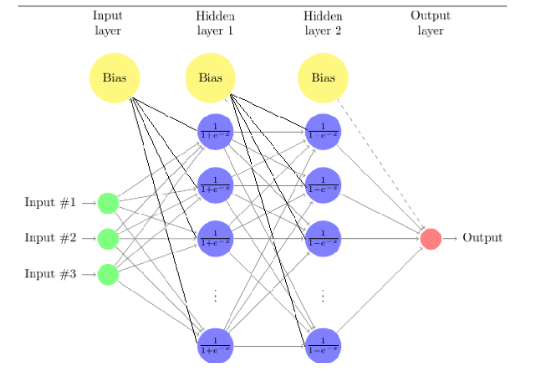
\includegraphics[width=1\textwidth]{chapters/chapter02/fig02/ann.PNG}
    \caption{Fully connected layers with bias term and Sigmoid activation functions}
    \label{fig:my_label}
\end{figure}
\subsection{Optimization in deep learning}
The choice of the optimizer in deep learning model can improve the results of the
models and reduces the timing from days to hours or minutes. The objective of all
optimizers is to reach the global minima where the cost function attains the least
possible value. The optimizer in the neural network is a parameter that could make the
difference between algorithm converging or exploding. There are a considerable number
of optimizers, here’s the most common used.
\subsubsection{Gradient Descent Optimizer}
he most popular and classic optimizer used in many optimization tasks , its role in
neural networks is to find the optimum values of a cost function. it is an optimization
algorithm, based on a convex function, that tweaks it’s parameters iteratively to minimize
a given function to its local minimum." A gradient measures how much the output of a
function changes if you change the inputs a little bit."\cite{art20}
\subsubsection{Stochastic gradient descent , Mini batch gradient descent}
Extension of the first described optimizer, is a popular algorithm for training a wide
range of different machine learning models such as SVM , ANN and logistic regression. Stochastic gradient descent maintains a single learning rate (termed alpha) for all
weight updates and the learning rate does not change during training, and it updates
the weights on the connections in each epoch. The motivation behind SGD is that in
very large redundant datasets , the gradient on the first half is almost identical to the
gradient on the second half. So instead of computing the full gradient, update the weights
using the gradient on the first half and then get a gradient for the new weights on the
second half. The extreme version of this approach updates weights after each case. It is
called Online\cite{c1}
\paragraph{Mini batches:}according to Goeffery hinton \cite{c1} the use of mini batches have proven
that it efficielntly helps in optimizing neural networks work better than the online
version in SGD, they offer many advantages :
\begin{itemize}
    \item Less computaion is used updating the weights.
    \item Computng the gradient for many cases simultaneously uses matrix-matrix muliplies
which are very efficient, especially on GPUs
\end{itemize}
\paragraph{Balanced mini batches:} while training the deep model, the weights of each class
should be the same, meaning that the number of samples ( training examples ) of each
class in the mini-batch should be the same.
\subsubsection{Adam}
Short to : adaptive moment estimation, Adam is an optimization algorithm that can
used instead of the classical stochastic gradient descent procedure to update network
weights iterative based in training data
\cite{art22} ,Computationally efficient. Little memory
requirements and Well suited for problems that are large in terms of data and/or parameters.
Empirical results demonstrate that Adam works well in practice and compares
favorably to other stochastic optimization methods
\cite{art22}
\subsubsection{RMSprop optimizer}
short for RootMean Squar prop. used for speeding the gradient descent optimization
process, is an unpublished optimizer proposed by Goeffrey hinton8 in \cite{c1} and well
recommended by him, appeared after rporp which has proven that it doesn’t work well with very large datasets \cite{c1}  RMSprop gave the ability to deal with larg datasets and works well with mini batches.
\subsection{Regularization for Deep Learning}
Deep neural networks with a large number of parameters and layers are very powerful
machine learning systems. However, overfitting is a serious problem in such networks.
Large networks are also slow to use, making it difficult to deal with overfitting by
combining the predictions of many different large neural nets at test time.
\subsubsection{Dropout}
The key idea is to randomly drop units (along with their connections) from the neural
network during training. This prevents units from co-adapting too much.
During training, dropout samples from an exponential number of different thinned
networks. At test time, it is easy to approximate the effect of averaging the predictions
of all these thinned networks by simply using a single unthinned network that has
smaller weights.\cite{art20} This significantly reduces overfitting and gives major improvements
over other regularization methods. Dropout is usually only applied after fully connected
layers, but not after convolutional layers as it usually increases the test error as pointed
out in \cite{art23}.
\begin{figure}[!h]
    \centering
    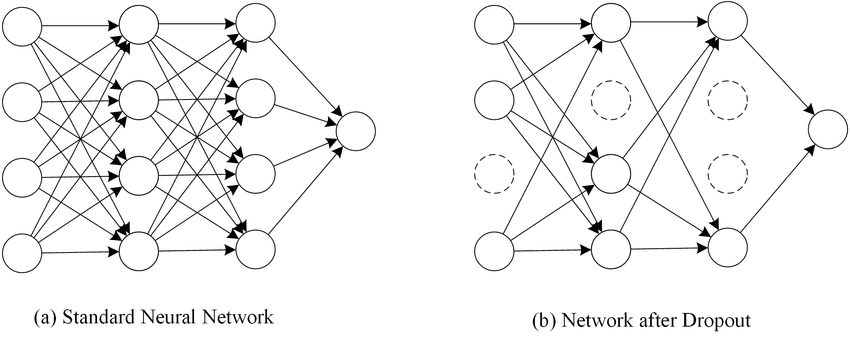
\includegraphics[width=1.1\textwidth]{chapters/chapter02/fig02/Dropout.png}
    \caption{Dropout a neural network}
    \label{fig:my_label}
\end{figure}
\subsubsection{Batch Normalization}
Batch normalization is one of the most exciting recent innovations in optimizing deep
neural networks \cite{art20}, if the batch norm is applied to a layer, it aims to normalize or standarise the ouptut value of the activation function by subtracting the batch mean
and dividing by the batch standard deviation, yet Andrew NG [44] recommends to apply
batch normalization before the activation function.
Batch normalization also allows each layer of a network to learn by itself a little bit more
independently of other layers.\cite{c2}
\cite{art24} \\

Batch Normalization reduces overfitting because it has a slight regularization effects.
Similar to dropout, it adds some noise to each hidden layer’s activations. Therefore, while
using batch normalization, this means we should use less dropout, which is a good thing
because we are not going to lose a lot of information. \cite{art24}
\subsubsection{Early stopping}
\label{Early stopping}
When training large models with sufficient representational capacity to overfit the
task, we often observe that training error decreases steadily over time, but validation
set error begins to rise again. Instead of running our optimization algorithm until we
reach a (local) minimum of validation error, we run it until the error on the validation
set has not improved for some amount of time.\cite{art20} When building a deep model, some
features are used to perfectly fit the model to the complex data. Generally there is no
rule to apply directly these parameteres, the developer, data scientist needs some times
to keep changing until the problem is converged. In the case of early stopping, we are
controlling the effective capacity of the model by determining how many steps it can take
to fit the training set.\cite{art25}
\subsubsection{Data augmentation}
Is a method of boosting the size of the training set, usually it works well when
the dataset isn’t efficiently large to be trained by a deep neural nets, Training deep
learning neural network models on more data can result in more skillful models, and
the augmentation techniques can create variations of the images that can improve the
ability of the fit models to generalize what they have learned to new images. This can
take several forms depending of the dataset. Usually done by taking the images and
make copies of them by scaling , cropping, rotating these images.\cite{art20}
\subsection{Model parameters}
When compiling and fitting the model to a given dataset , some parameters needs to
be specified , here are some of them mentioned briefly.
\subsubsection{learning rate}
The learning rate is introduced as a constant (usually very small), in order to force
the weight to get updated very smoothly and slowly (to avoid big steps and chaotic
behaviour).
Geoffery hinton explain how the learning rate parameter is ajusted.\cite{c1} If the error
keeps going worse or oscillates wildly, reduce the learning rate.
If the error is falling fairly consistently but slowly, increase the learning rate.
Turn down the learning rate when the error stops decreasing.
\subsubsection{epoch}
One Epoch is when the entire dataset is passed forward and backward through the
neural network only once. Epoch parameters refers to how many times the models aims
to use the complete dataset for training.
\subsubsection{Batch}
While training, the dataset is divided to a number of batches/parts, big mini-batches
are more computationally efficient.

\subsubsection{Batch size}
Total number of training examples present in a single batch.

\subsubsection{loss functions}
Is a performance metric on how well the neural net manages to reach its goal of
generating outputs as close as possible to the desired values loss = sum of squares
[Desired output-actual output].where the robustness of model increases along with the
decrease of the value of loss function. The goal of the model is to minimize this loss

\paragraph{Categorical crossentropy} It is a Softmax activation plus a Cross-Entropy loss. If we
use this loss, we will train a CNN to output a probability over the C classes for each image. It is used for multi-class classification. Compares the predicted label and true
label and calculates the loss.
\subsubsection{Activation functions}
Activation functions are an extremely important feature of the artificial neural
networks. They basically decide whether the information( Weight Å bias ) received by
the neuron(from the previous layer) is enough for the neuron to be activated or not. This
transformed output is then sent to the next layer of neurons as input.

\paragraph{Why activation function ?} If the model is trained without an activation function,
the information shared between neurons in different layers are following a simple
linear transformation, while problem solved by the deep neural nets are generally
very complicated, this where the activation functions works, they apply a non linear
transformation of the input signal. A neural network without an activation function is
just a linear regression model. and since the activation function applies a non linear
transformations, they help the backpropagation task.

\paragraph{Sigmoid} A very popular activation function that has proven solving the two-classes
classification task since it produces values between 0 and 1. if the instance value’s weight
is minthreshold, the class is negative and so on.

\paragraph{ReLU} Stands for Rectified Linear Unit, most widely used activation function in the
field of neural networks, is a non linear function.
The major advantage of ReLU is that it does not activate all the neurons at the same
time, meaning that, if the input is negative it will convert it to zero(in other words it
returns the highest value between 0 and the weight+bias ) and the neuron does not get
activated, producing few neurons to be activated at a time.
\begin{figure}[!h]
    \centering
    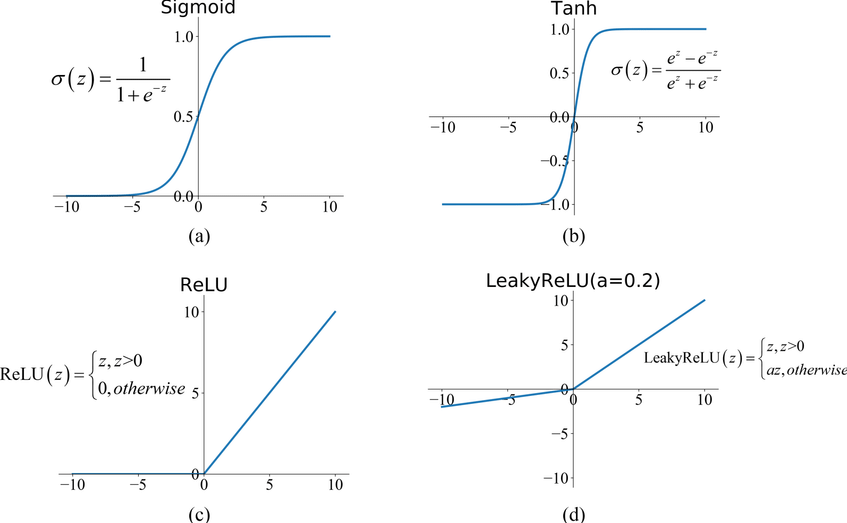
\includegraphics[width=0.85\textwidth]{chapters/chapter02/fig02/act.PNG}
    \caption{Caption}
    \label{fig:my_label}
\end{figure}

\paragraph{Softmax} An enhancement of sigmoid function, it enables the multi classification
tasks,the softmax function would squeeze the outputs for each class between 0 and 1 and
would also divide by the sum of the outputs. This essentially gives the probability of the
input being in a particular class.

\paragraph{TanH} Hyperbolic tangent is a non linear transformation function, works similar to
the sigmoid function but is symmetric over the origin. it ranges from -1 to 1.

\section{Convolutional neural network}
Proposed by Yann Lecun \cite{art26} is considered as the most used type of Artificial Neural
Nets in image and video recognition , image classification, computer vision and natural
language processing.
Convolutional networks are simply neural networks that use
convolution in place of general matrix multiplication in at least one of their layers.
Convolutional networks have played an important role in the history of deep learning.
They are a key example of a successful application of insights obtained by studying the
brain to machine learning applications. They were also some of the first deep models to
perform well, long before arbitrary deep models were considered viable.\cite{art20}\\

A typical layer of a convolutional network consists of three stages. In the first stage,
the layer performs several convolutions in parallel to produce a set of linear activations.
In the second stage, each linear activation is run through a nonlinear activation function,
such as ReLU. This stage is sometimes called the detector stage. In the third stage, we use
a pooling function to modify the output of the layer further.\cite{art20} 3D volumes of neurons.
Convolutional Neural Networks take advantage of the fact that the input consists of
images and they constrain the architecture in a more sensible way. In particular, unlike a
regular Neural Network, the layers of a ConvNet have neurons arranged in 3 dimensions:
width, height, depth. \vspace{4mm} \\
Simple ConvNet is a sequence of layers, and every layer of a ConvNet transforms one
volume of activations to another through a differentiable function. We use three main
types of layers to build ConvNet architectures: Convolutional Layer, Pooling Layer, and
Fully-Connected Layer.

\subsection{Convolution layer}
The Convolution layer(or Conv layer) is the core building block of a Convolutional
Network that does most of the computational heavy lifting. Most generally, we can think
of a CNN as an artificial neural network that has some type of specialization for being
able to pick out or detect patterns. This pattern detection is what makes CNNs so useful
for image analysis. \vspace{4mm} \\
Convolutional layer receives input, transforms the input by doing convolution operation,
and then outputs the transformed input to the next layer.
The inputs to convolutional layers are called input channels, that have three channels
(Width , Hight , depth). \vspace{4mm} \\
With a convolutional layer, the transformation that occurs is called a convolution
operation. This is the term that’s used by the deep learning community anyway. Mathematically,
the convolution operations performed by convolutional layers are actually
called cross-correlations. \cite{art20}

\subsubsection{Convolution operation}
Convolution is a mathematical operation to merge two sets of information. In our
case the convolution is applied on the input data using a convolution filter to produce a
feature map. The convolution operation is performed by sliding (i.e convolving ) this filter
over the image. At every location, we do element-wise matrix multiplication and sum
the result. This sum goes into the feature map. the layers are organized in 3 dimensions:
width, height and depth
\subsubsection{Filters}
he Conv layer’s parameters consist of a set of filters also known as kernels. the
filters are especially designed to detect whether or not the image does contain any such
characteristics. Every filter is small spatially (along width and height), but extends
through the full depth of the input volume , meaning that it should have the same depth
of the input.
\subsection{Pooling layer}
Also called features detector, Its function is to progressively reduce the spatial size of
the representation in order to reduce the amount of parameters and computation in the
network, hence to control overfitting. In image classifications task \cite{art20} , pooling reduces
the dimonsiality of the image by the reducing the number of pixels in the output from
the previous convolutinal layer. \vspace{4mm}\\
Pooling helps to make the representation become approximately invariant to small
translations of the input. Invariance to translation means that if we translate the input
by a small amount, the values of most of the pooled outputs does not change. \cite{art20}, \vspace{4mm} \\
Many types of Pooling layers were proposed \cite{art27}, these are the most common used :
\subsubsection{Max pooling}
uses the maximum value from each cluster of neurons at the prior
layer. main goal of max poooling is to capture the main feauters and give them high
weights , when these features are found while filtering the image ( in the convoloution
phase ) these feautres are returened (because they have the maximum value ) while the
no-important features(those who have less value are neglected)  \cite{c2}

\subsubsection{Average pooling}
uses the average value from clusters of neurons at the prior layer
\begin{figure}[!h]
    \centering
    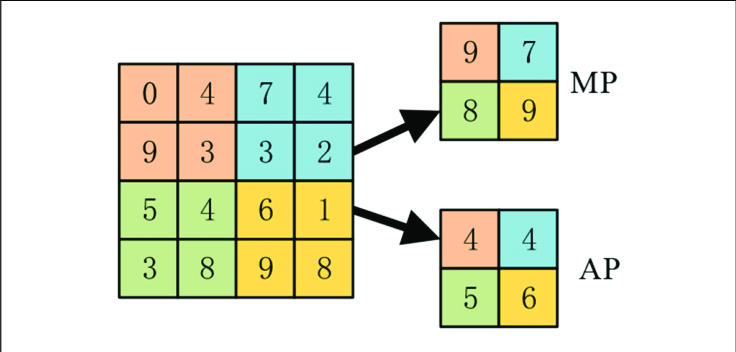
\includegraphics[width=1\textwidth]{chapters/chapter02/fig02/pol.png}
    \caption{ Max Pooling & Average Pooling}
    \label{fig:my_label}
\end{figure}

\subsection{Padding}
As already mentioned in the previous subsection, each convolution layer is applied
with a filter that has a dimension, When a filter convolves a given input channel, it gives
us an output channel. This output channel is a matrix of pixels with the values that
were computed during the convolutions that occurred on the input channel. When this
happens, the dimensions of our image are reduced.\vspace{4mm} \\
This means that when this 3 x 3 filter finishes convolving this 4 x 4 input, it will give
us an output of size 2 x 2 This issue is resolved by the Zero padding: Zero padding is a
technique that allows us to preserve the original input size. With each Conv layer added
to the strucutre it is possible to specify whether or not to use padding. Zero padding
refers to the addition of border of pixels with zreo values arround the edge of the image.

\subsubsection{Same Padding}
This means that we want to pad the original input before we convolve
it so that the output size is the same size as the input size.

\subsubsection{Valid Padding} This just means no padding. If we specify valid padding, that means
our convolutional layer is not going to pad at all, and our input size won’t be maintained.
\section{Attention Mechanism}
The idea behind the attention mechanism was to permit the model to utilize the most relevant parts of the input sequence in a flexible manner,by providing an additional focus on a specific component
is able to learn the association between them,
Attention Mechanism is also an attempt to implement the same action of selectively concentrating on a few relevant things, while ignoring others in deep neural networks.\cite{art44}


\subsection{Convolutional Block Attention Module (CBAM)}

Convolutional Block Attention Module (CBAM)
a simple yet effective attention module for feed-forward convolutional
neural networks. Given an intermediate feature map, our module sequentially infers attention maps along two separate dimensions, channel
and spatial, then the attention maps are multiplied to the input feature
map for adaptive feature refinement. Because CBAM is a lightweight and
general module, it can be integrated into any CNN architectures\cite{art44}
\begin{figure}[H]
    \centering
    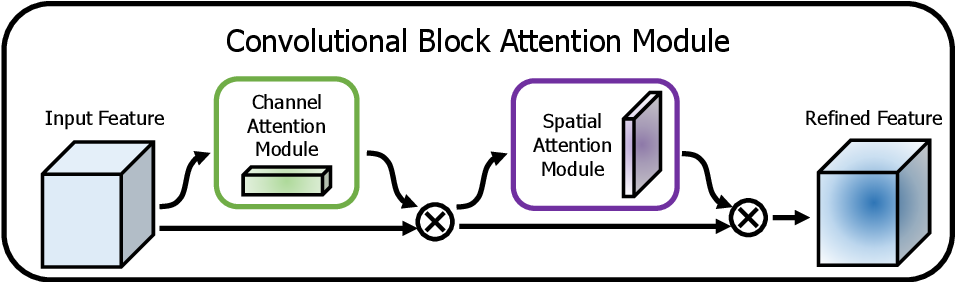
\includegraphics[width=0.85\textwidth]{chapters/chapter02/fig02/cbam.PNG}
    \caption{Convolutional Block Attention Module (CBAM)}
\end{figure}
CBAM contains two sequential sub-modules called the Channel Attention Module (CAM) and the Spatial Attention Module (SAM)
\subsubsection{Channel Attention Module (CAM)}
Channel Attention Module (CAM) focuses on ‘what’ is
meaningful given an input image,it
decomposes the input tensor into 2 subsequent vectors of dimensionality (c × 1 × 1). One of these vectors is generated by GAP while the other vector is generated by Global Max Pooling (GMP). Average pooling is mainly used for aggregating spatial information, whereas max pooling preserves much richer contextual information in the form of edges of the object within the image which thus leads to finer channel attention. Simply put, average pooling has a smoothing effect while max pooling has a much sharper effect.\cite{art44}
\subsubsection{Spatial Attention Module (SAM)}
Spatial Attention Module (SAM) focuses on ‘where’ is an informative part. is comprised of a three-fold sequential operation. The first part of it is called the Channel Pool, where the Input Tensor of dimensions (c × h × w) is decomposed to 2 channels, i.e. (2 × h × w), where each of the 2 channels represent Max Pooling and Average Pooling across the channels. This serves as the input to the convolution layer which output a 1-channel feature map, i.e., the dimension of the output is (1 × h × w).\cite{art44}

\begin{figure}[H]
    \centering
    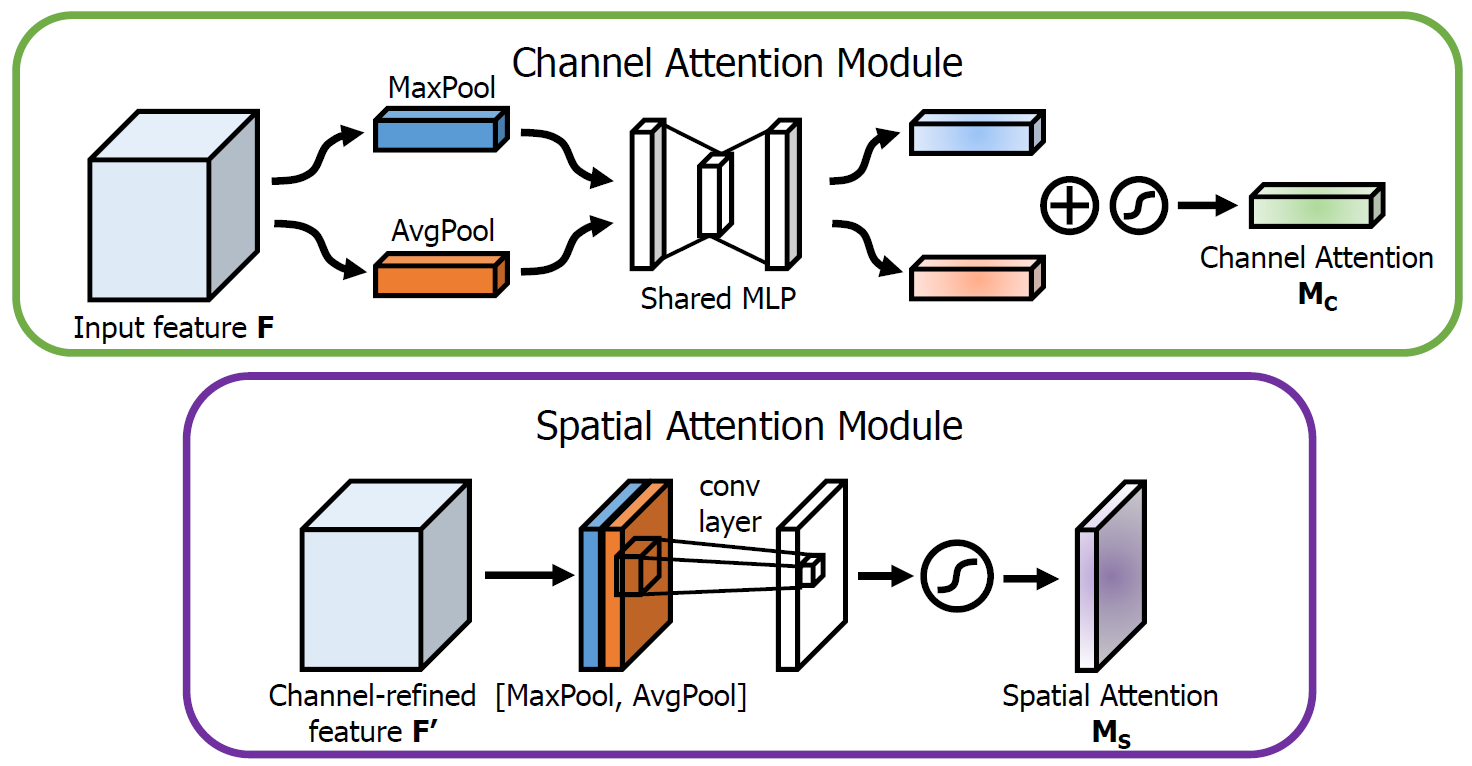
\includegraphics[width=0.85\textwidth]{chapters/chapter02/fig02/cbam2.PNG}
    \caption{Channel Attention Module (CAM) & Spatial Attention Module (SAM)}
\end{figure}

\subsection{Gradient-weighted Class Activation Mapping (Grad-CAM)}
For the qualitative analysis, we apply the Grad-CAM \cite{art45} 
is a technique for producing visual explanations for decisions from a large class of CNN-based models, making them more transparent.
 Grad-CAM is a recently proposed
visualization method which uses gradients in order to calculate the importance
of the spatial locations in convolutional layers. As the gradients are calculated with respect to a unique class, Grad-CAM result shows attended regions clearly.
By observing the regions that network has considered as important for predicting
a class, we attempt to look at how this network is making good use of features.


\section{Transfer learning}
\label{Transfer learning}
The term of transfer learning is related to use a pretrained model, regarding the
weights and the parameters, and fine tune it to solve a specific image classification task.
\subsection{Transfer learning VS traditional learning}
Traditional learning methods build a new classifier from scratch for each classification
task.Transfer learning applies knowledge from a source classifier to simplify the
construction of a classifier for a new, target tasks. \cite{book5}

\subsection{ImageNet}
ImageNet is an image database that contains 14,197,122 images and more than 1,000
classes, and can be freely accessed in ImageNet website \cite{art28}
Since 2010, the ImageNet project runs an annual software contest, the ImageNet Large Scale Visual Recognition Challenge (ILSVRC), where software programs compete to Correctly classify and detect objects and scenes.

\subsection{Pretrained Model}
here we presents some famous pretrained model on ImageNet dataset and
their architecture.
In the pretrained model the weights and parameters of a network that has been trained
on a imageNet dataset and saved for further use of image classification tasks.

\subsubsection{VGG-16}
Stands for Visual Geometry Group with pushing the depth to 16 weight layers ,is a
pretrained VERY DEEP Convolutional networks for large-scale image recognition thatwas proposed by the VGG group \cite{art30} ,University of Oxford, while their participation in
ImageNet LSVRC-2014 where they secured the first and second place for image classification
and localization. The model contains 138M parameters and 294,9112 weights.

\begin{figure}[!h]
    \centering
    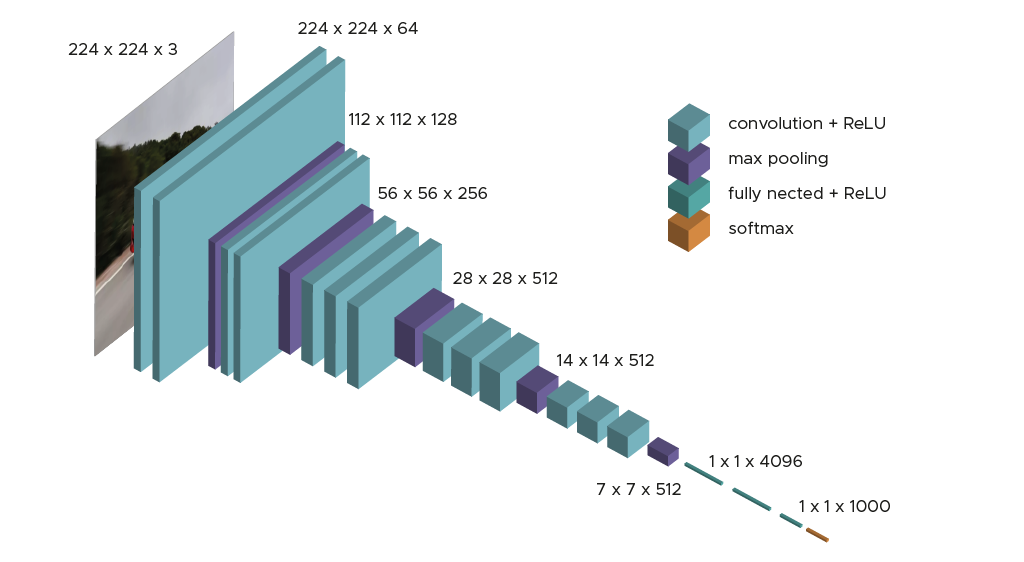
\includegraphics[width=1\textwidth]{chapters/chapter02/fig02/vgg16.png}
    \caption{ VGG16 architecture}
    \label{fig:my_label}
\end{figure}
\subsubsection{VGG-19}
The visual geometry group network (VGGNet) is a deep neural network with a multilayered
operation. The VGGNet is based on the CNN model and is applied on the ImageNet dataset. VGG-19
is useful due to its simplicity as 3 × 3 convolutional layers are mounted on the top to increase with
depth level \cite{art41}
The number 19 stands for the number
of layers with trainable weights, 16 Convolutional layers and 3 Fully Connected layers. 



\subsubsection{Inception}
The Inception deep convolutional architecture was introduced as GoogLeNet in
(Szegedyet al.)\cite{art31}, here named Inception-v1. Later the Inception architecture was
refined in various ways, first by the introduction of batch normalization (Ioffe and
Szegedy 2015) (Inception-v2). Later by additional factorization ideas in the third iteration
(Szegedyet al. 2015b) which will be referred to as Inception-v3 in this report.is a
pretrained model that contains 7 million parameters and 42-layer deep learning network.

\subsubsection{Xception}
The Xception architecture \cite{art42}, introduced by
Francois Chollet, is an extension of the Inception architecture. This architecture is a linear stack of depthwise
separable convolution layers with residual connections.
\begin{figure}[!h]
    \centering
    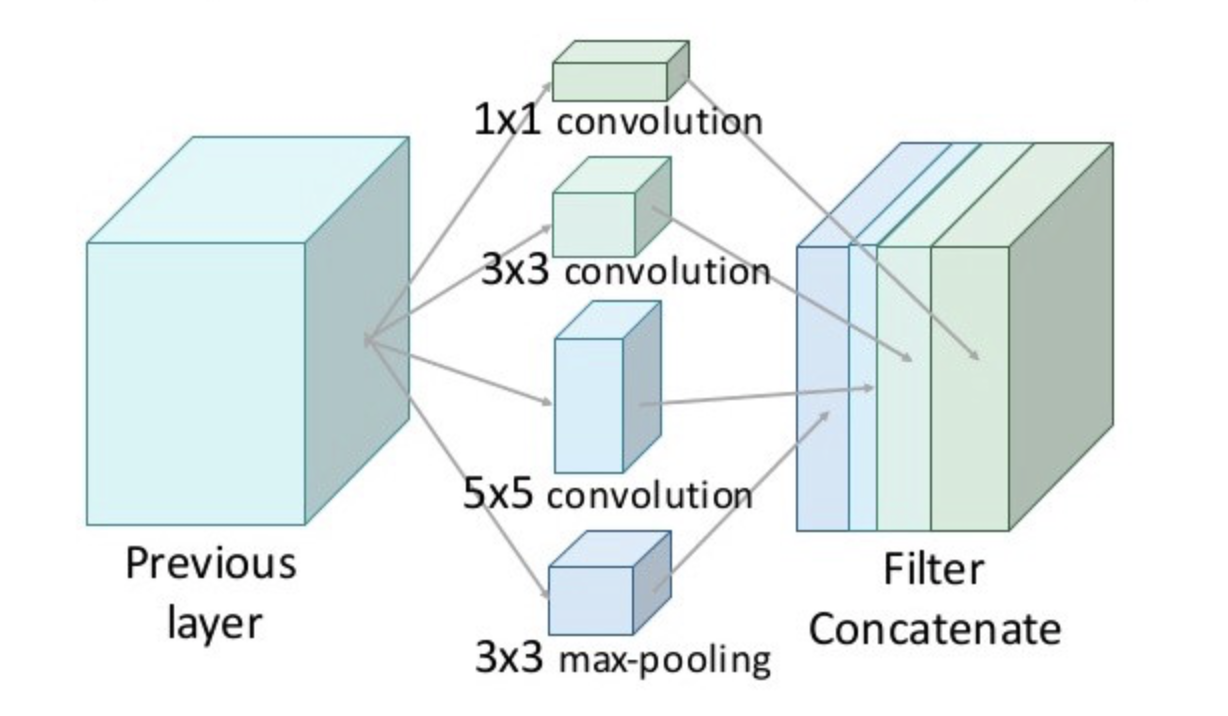
\includegraphics[width=1\textwidth]{chapters/chapter02/fig02/xception.png}
    \caption{ Xception architecture}
    \label{fig:my_label}
\end{figure}

\subsubsection{ResNet}
ResNet is a short name for Residual Network proposed in \cite{art32}. As the name of the
network indicates, the new terminology that this network introduces is residual learning.
Residual nets with a depth of up to 152 layers—8x deeper than VGG nets but still having
lower complexity. An ensemble of these residual nets achieves 3.57 error on the ImageNet
test set. This result won the 1st place on the ILSVRC 2015 classification task.
\begin{figure}[!h]
    \centering
    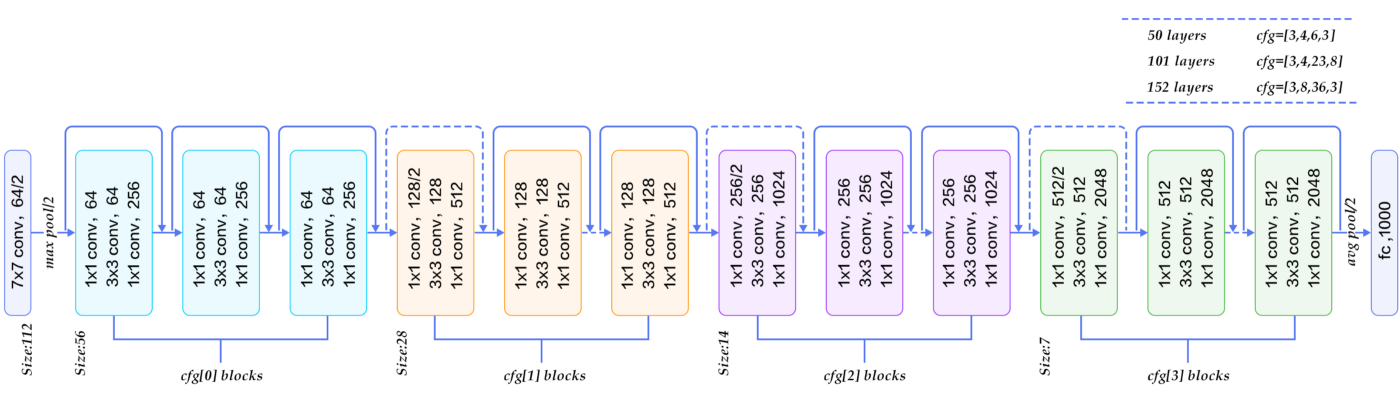
\includegraphics[width=1\textwidth]{chapters/chapter02/fig02/resnet50.png}
    \caption{ ResNet architecture}
    \label{fig:my_label}
\end{figure}

\subsubsection{MobileNet V2}
MobileNetV2 is a convolutional neural network architecture that seeks to perform well on mobile devices. It is based on an inverted residual structure where the residual connections are between the bottleneck layers. The intermediate expansion layer uses lightweight depthwise convolutions to filter features as a source of non-linearity. As a whole, the architecture of MobileNetV2 contains the initial fully convolution layer with 32 filters, followed by 19 residual bottleneck layers. \cite{art40}

\begin{figure}[!h]
    \centering
    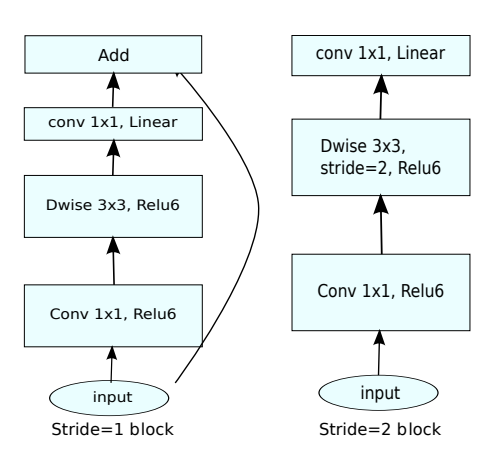
\includegraphics[width=1\textwidth]{chapters/chapter02/fig02/mobilenet.png}
    \caption{ MobileNetV2 architecture}
    \label{fig:my_label}
\end{figure}
\subsubsection{EfficientNet}
EfficientNet is a convolutional neural network architecture and scaling method that uniformly scales all dimensions of depth/width/resolution using a compound coefficient to scale up models in a simple but effective manner. Instead of randomly scaling up width, depth or resolution, compound scaling uniformly scales each dimension with a certain fixed set of scaling coefficients. Using the scaling method and AutoML, the authors of efficient developed seven models of various dimensions, which surpassed the state-of-the-art accuracy of most convolutional neural networks, and with much better efficiency.
EfficientNet is based on the baseline network developed by the neural architecture search using the AutoML MNAS framework
The architecture uses a mobile inverted bottleneck convolution similar to MobileNet V2.
EfficientNets have been the State-of-the-art for high quality and quick image classification. \cite{art43}
The number of layers in EfficientNet-B0 is 237 and in EfficientNet-B7 the total comes out to 813!

\subsubsection{DenseNet}
DenseNet (Dense Convolutional Network) is an architecture that focuses on making the deep learning networks go even deeper, but at the same time making them more efficient to train,that utilises dense connections between layers, through Dense Blocks, where we connect all layers (with matching feature-map sizes) directly with each other,the first layer is connected to the 2nd, 3rd, 4th for example,DenseNets have several compelling advantages: they alleviate the vanishing-gradient problem, strengthen feature propagation, encourage feature reuse, and substantially reduce the number of parameters.\cite{art47}

\begin{figure}[!h]
    \centering
    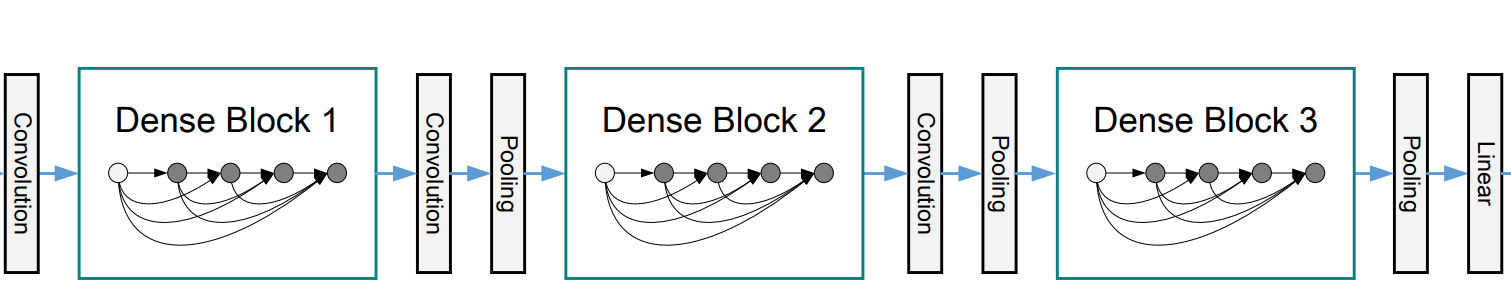
\includegraphics[width=1\textwidth]{chapters/chapter02/fig02/densnet.png}
    \caption{ DenseNet architecture}
    \label{fig:my_label}
\end{figure}
 
 
  

\subsubsection{Fine-tuning}
Fine-tuning, in general, means making small adjustments to a process to achieve the desired output or performance. Fine-tuning deep learning involves using weights of a previous deep learning algorithm for programming another similar deep learning process. Weights are used to connect each neuron in one layer to every neuron in the next layer in the neural network. The fine-tuning process significantly decreases the time required for programming and processing a new deep learning algorithm.

\newpage

\section{Vision Transformer}
The Vision Transformer, or ViT, is a model for image classification that employs a Transformer-like architecture over patches of the image. An image is split into fixed-size patches, each of them are then linearly embedded, position embeddings are added to retain positional information, and the resulting sequence of vectors is fed to a standard Transformer encoder. In order to perform classification, the standard approach of adding an extra learnable “classification token” to the sequence is used, Internally, the transformer learns by measuring the relationship between input token pairs,Recently, Vision Transformers (ViT) have achieved highly competitive performance in benchmarks for several computer vision applications, such as image classification, object detection, and semantic image segmentation.\cite{art46} \\

The overall architecture of the vision transformer model is given as follows in a step-by-step manner \cite{w10}:
\begin{enumerate}
    \item Split an image into patches (fixed sizes)
    \item Flatten the image patches
    \item Create lower-dimensional linear embeddings from these flattened image patches
    \item Include positional embeddings
    \item Feed the sequence as an input to a state-of-the-art transformer encoder
    \item Pre-train the ViT model with image labels, which is then fully supervised on a big dataset
    \item Fine-tune on the downstream dataset for image classification
\end{enumerate}
The transformer encoder includes  \cite{w10}:
\begin{itemize}
    \item \textbf{Multi-Head Self Attention Layer (MSP):} This layer concatenates all the attention outputs linearly to the right dimensions. The many attention heads help train local and global dependencies in an image.

    \item \textbf{ Multi-Layer Perceptrons (MLP) Layer:} This layer contains a two-layer with Gaussian Error Linear Unit (GELU).
    \item \textbf{Layer Norm (LN):} This is added prior to each block as it does not include any new dependencies between the training images. This thereby helps improve the training time and overall performance.
\end{itemize}

\begin{figure}[H]
    \centering
    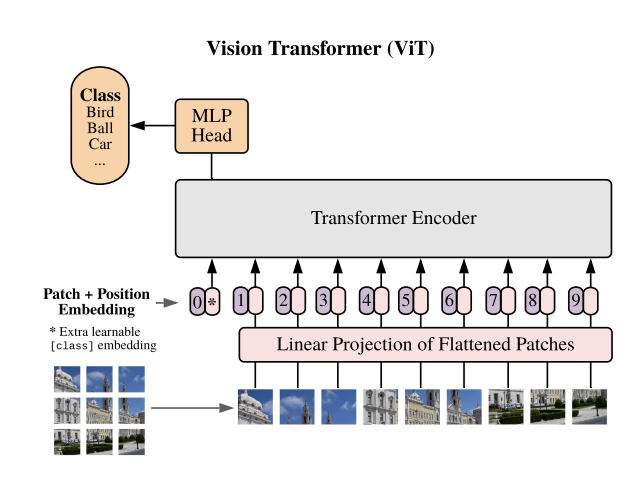
\includegraphics[width=1\textwidth]{chapters/chapter02/fig02/vit.png}
    \caption{ Vision Transformer architecture}
\end{figure}

\section{Related work using deep learning}
This section mentions the previous works dealing with classifying Plant leaf diseases images
using deep convolutional neural nets and pretrained models.
\begin{itemize}
    \item Sardogan \textit{et al} \cite{art33}  have proposed a very deep CNN network architecture contained 4 CONV blocks and 1 FC layers. Max pooling was placed after the 2nd, 3rd and the 4th CONV blocks.A 9x9 filter has been used in the first and second convolutions, and a 5x5 filter has been used in the third and fourth convolutions. After these implications, three different 3x3 matrices have been obtained for R, G and B channels separately. The FC layer included 27 neurons. A Relu layer was placed at the end of each CONV. \\
    The experiments showed that the average prediction accuracy of CNN-based method was 86\%. 
    \item Mohanty \textit{et al} \cite{art34} evaluate the applicability of deep convolutional neural networks for the classification problem. Focusing on two popular architectures, namely AlexNet \cite{art29}, and GoogLeNet (Szegedy et al., 2015). In case of transfer learning, they re-initialize the weights of layer fc8 in case of AlexNet, and of the loss {1,2,3}/classifier layers in case of GoogLeNet. 
    Then, when training the model, they do not limit the learning of any of the layers, as is sometimes done for transfer learning. In other words, the key difference between these two learning approaches (transfer vs. training from scratch) is in the initial state of weights of a few layers, which lets the transfer learning approach exploit the large amount of visual knowledge already learned by the pre-trained AlexNet and GoogleNet models extracted from ImageNet \cite{art31}. To summarize, they have a total of 60 experimental configurations.\\
    The trained model achieves an accuracy of 99.35\% on a held-out test set.
    \item Chen, J \textit{et al} \cite{art35} inspired by the performances, the VGGNet with the Inception module is selected in our approach. The conventional VGGNet was enhanced by replacing its last convolutional layers with an additional convolutional layer of 3 × 3 × 512, then the batch normalization (BN) was added on the convolutional layer and the Swish activation function is used to directly replace ReLU. Furthermore, they modified the conventional VGGNet by replacing its full connection layers with a global pooling layer, and two Inception modules, as stated before, are introduced in the VGGNet to improve the feature extraction ability of the new network, namely, INC-VGGN. and it is of little value to utilize Inception to extract these features. Therefore, the Conv1-1 to Pool3 layers of the VGGNet are preserved and the subsequent layers of VGGNet, Conv5-1 to Conv5-3, are replaced with two Inception modules and one added BN convolutional layer, in which the Swish is used as the activation function instead of the ReLU. a convolutional layer with batch normalization and Swish is added behind Pooling3, and then the two Inception modules composed of Inception and Concat are conducted to enhance the multi-scale feature extraction ability of the network.Finally, a global pooling layer instead of fully-connected layers are added after the second Inception module and followed by a Softmax classifier.\\
    The experiments showed that the average prediction accuracy was no less than 91.83\% on the public dataset.

    \item Another paper on classifying Plant-Leaf Diseases using deep learning methods by Liu, B \textit{et al} \cite{art36} deep convolutional neural network model is proposed to identify apple leaf diseases. they proposed an architecture where the first convolutional layer is designed to be 96 kernels of size 9 × 9 × 3, which is different from the Symmetry 2018, 10, 11 7 of 16 first convolutional layer’s kernel size of 11 × 11 × 3 in the standard AlexNet. The second convolutional layer filters the noise with 256 kernels of size 5 × 5 × 48, response-normalization layers follow the first two convolutional layers, which are themselves followed by max-pooling layers. The third convolutional layer has 384 kernels with a size of 3 × 3 × 256 connected to the (normalized, pooled) outputs of the second convolutional layer. The fourth layer is filtered with 384 kernels of size 3 × 3 × 192, and the fifth layer has 256 kernels with a size of 2 × 2 × 192 to improve the ability to extract small features, which is also different from the standard AlexNet, and is then followed by a max-pooling layer. After AlexNet Precursor, an architecture named Cascade Inception is designed including two max-pooling layers and two Inception structures. The first max-pooling layer is applied to filter the noise of feature maps generated by AlexNet Precursor, and the two Inceptions then extract the optimal discrimination features from multidimension analysis. Feature maps before the first Inception are input into the second Inception’s concatenation layer, which prevents some of the features being filtered by these two Inceptions. Meanwhile, the sixth convolutional layer followed by the Cascade Inception has 4096 kernels with a size of 1 × 1 × 736, which replaces the first two fully connected layers of the standard AlexNet. The fully connected layer is adjusted to predict four classes of apple leaf diseases, and the final layer is a four-way Softmax layer.\\ 
    the experimental results show that the proposed disease identification approach based on the convolutional neural network achieves an overall accuracy of 97.62\%.
    \item Published By Brahimi M, Boukhalfa K and Moussaoui A \cite{art37} Pre-taining phase: in this phase they train deep architectures on a large dataset like ImageNet using powerful machines. The objective of this phase is the initialization of network weights for the next phase.
    Training (fine-tuning): they fine-tune the resulted network from the first phase. Also, they replace the output layer of the pre-tained networks (ImageNet contains 1000 classes) by a new output layer having nine classes (nine diseases of tomato). They have used two CNN models (AlexNet (Alex, Sutskever, and Hinton 2012) and GoogleNet (Szegedy et al. 2015)). \\
    The obtained results are encouraging, reaching 99.18\% of accuracy
\end{itemize}
\subsection{Related works summarized}
\begin{table}[!h]
	\begin{tabular}{@{}|p{3cm}|p{1.5cm}|p{4cm}|p{4cm}|p{3cm}|@{}}
		\toprule
		 \center \textbf{Paper} & \center \textbf{Year} & \center \textbf{ Data} & \center \textbf{Classification Methods} & \begin{center}  \textbf{Accuracy}
	    \end{center} \\ \midrule
      
       \center \textbf{ \cite{art6} } & \center  2016  &  \center  Grape leaves images & \center SVM	&  \begin{center} 88.89 \%  \end{center}\\
       \midrule\midrule
       
       \center \textbf{ \cite{art7} } & \center  2013  &  \center  9 Types of plants(banana, beans, jackfruit, lemon, mango, potato, tomato, guava and sapota) & \center SVM	&  \begin{center} 94.74 \%  \end{center}\\
       \midrule\midrule
       
       \center \textbf{ \cite{art8} } & \center  2018  &  \center  Papaya leaves images & \center Random Forest	&  \begin{center} 70.14  \%  \end{center}\\
       \midrule\midrule
       
       \center \textbf{ \cite{art9} } & \center  2021  &  \center  Maize Leaf Disease Dataset & \center Random Forest	&  \begin{center} 80.68  \%  \end{center}\\
       \midrule\midrule
       
       \center \textbf{ \cite{art10} } & \center  2004  &  \center  Soil texture, weather variables and tillage practices & \center Logistic Regression	&  \begin{center} 78.5 and 77.8  \%  \end{center}\\
       \midrule\midrule
       
       \center \textbf{ \cite{art11} } & \center  2020  &  \center  PlantVillage dataset & \center Logistic Regression	&  \begin{center}  97.7 \%  \end{center}\\
       \midrule\midrule
       
       \center \textbf{ \cite{art12} } & \center  2017  &  \center  Original cassava dataset & \center KNN	&  \begin{center}  96.76 \%  \end{center}\\
       \midrule\midrule
       
       \center \textbf{ \cite{art13} } & \center  2019  &  \center  Groundnut leaves images & \center KNN	&  \begin{center}   /  \end{center}\\
       \midrule
      
    \end{tabular}
	

\end{table}
\newpage
\begin{table}[!h]
	\begin{tabular}{@{}|p{1.5cm}|p{1.5cm}|p{4.5cm}|p{4cm}|p{3cm}|@{}}
		\toprule
		 \center \textbf{\cite{art15}} & \center \textbf{2020} & \center \textbf{ Plant leaf images (1000 images)} & \center \textbf{Decision Tree } & \begin{center}  \textbf{96 \%}
	    \end{center} \\ \midrule
	    
	    \center \textbf{\cite{art16}} & \center \textbf{2019} & \center \textbf{ Rice leaf images(480 images)} & \center \textbf{Decision Tree } & \begin{center}  \textbf{97.9167  \%}
	    \end{center} \\ \midrule
	    
	    \center \textbf{\cite{art19}} & \center \textbf{2020} & \center \textbf{ Original cassava dataset} & \center \textbf{Naïve Bayes  } & \begin{center}  \textbf{77.46   \%}
	    \end{center} \\ \midrule
	    
	    \center \textbf{\cite{art33}} & \center \textbf{2018} & \center \textbf{ Tomato leaves images 500} & \center \textbf{CNN} & \begin{center}  \textbf{86  \%}
	    \end{center} \\ \midrule
	    
	    \center \textbf{\cite{art34}} & \center \textbf{2016} & \center \textbf{ PlantVillage dataset} & \center \textbf{CNN, AlexNet and GoogleNet} & \begin{center}  \textbf{99.35  \%}
	    \end{center} \\ \midrule
	    
	    \center \textbf{\cite{art35}} & \center \textbf{2020} &  \textbf{  \begin{itemize}
	        \item Public dataset: plantVillage dataset
	        \item collected dataset: rice and maize image datasets \end{itemize}    } & \center \textbf{Cnn(VGGNet)} & \begin{center}  \textbf{91.83 \%}
	    \end{center} \\ \midrule
	    
	    \center \textbf{\cite{art36}} & \center \textbf{2017} & \center \textbf{ 13,689 diseased apple leaves images} & \center \textbf{CNN(AlexNet)} & \begin{center}  \textbf{97.62  \%}
	    \end{center} \\ \midrule
	    
	    \center \textbf{\cite{art37}} & \center \textbf{2017} & \center \textbf{ Images of tomato leaves from plantVillage } & \center \textbf{CNN,AlexNet and GoogleNet} & \begin{center}  \textbf{99.18  \%}
	    \end{center} \\ \midrule

\end{tabular}
\caption{List of various Related Works and its Results}	
\end{table}

\newpage


\section{Object Detection}
Object detection involves detecting instances of objects from one or several classes in an image. \cite{inbook1}

\subsection{YOLO}
The ‘You Only Look Once’ v3 (YOLOv3) method is among the most widely used deep
learning-based object detection methods. It uses the k-means cluster method to estimate the initial
width and height of the predicted bounding boxes. With this method, the estimated width and height
are sensitive to the initial cluster centers, and the processing of large-scale datasets is time-consuming.
In order to address these problems, a new cluster method for estimating the initial width and height
of the predicted bounding boxes has been developed. Firstly, it randomly selects a couple of width
and height values as one initial cluster center separate from the width and height of the ground
truth boxes. Secondly, it constructs Markov chains based on the selected initial cluster and uses
the final points of every Markov chain as the other initial centers. In the construction of Markov
chains, the intersection-over-union method is used to compute the distance between the selected
initial clusters and each candidate point, instead of the square root method. Finally, this method
can be used to continually update the cluster center with each new set of width and height values,
which are only a part of the data selected from the datasets. Our simulation results show that the new
method has faster convergence speed for initializing the width and height of the predicted bounding
boxes and that it can select more representative initial widths and heights of the predicted bounding
boxes. Our proposed method achieves better performance than the YOLOv3 method in terms of
recall, mean average precision, and F1-score. \cite{art38}


\section{Summary}[!h]
